%% ---------------------------------------------------------------------------
%% Small-model comparison: BLADE vs.\ ITI on Qwen3-4B and Llama-3.2-3B-Instruct
%% ---------------------------------------------------------------------------

\begin{figure*}[t]
  \centering
  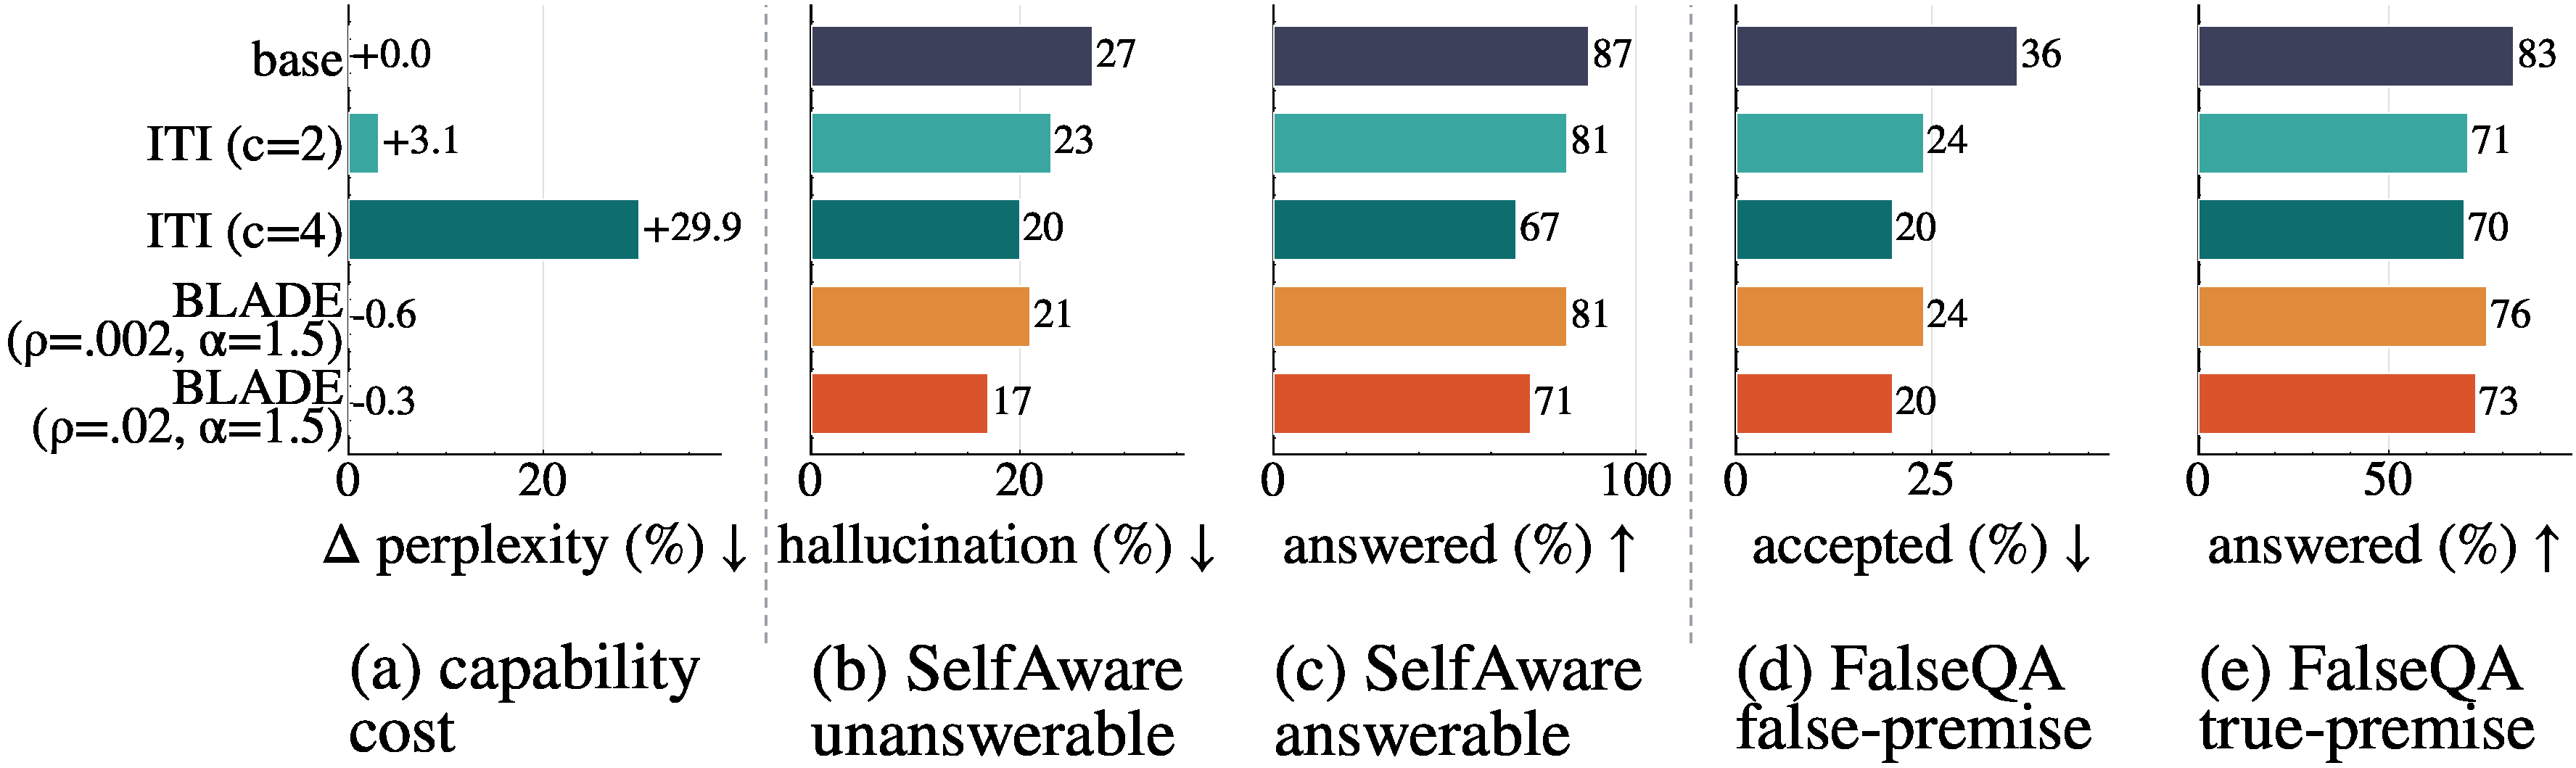
\includegraphics[width=\textwidth]{figures/uncertainty_method_cmp_qwen.pdf}
  \caption{\textbf{Qwen3-4B: BLADE vs.\ ITI}~\citep{li2023iti} on the uncertainty behaviors.
  (a)~C4 $\Delta$-perplexity, (b)~SelfAware unanswerable hallucination, (c)~SelfAware answerable answered,
  (d)~FalseQA false-premise accepted, (e)~FalseQA true-premise answered; lower is better in (a,\,b,\,d),
  higher in (c,\,e).}
  \label{fig:umc-qwen4b}
\end{figure*}

\begin{figure*}[t]
  \centering
  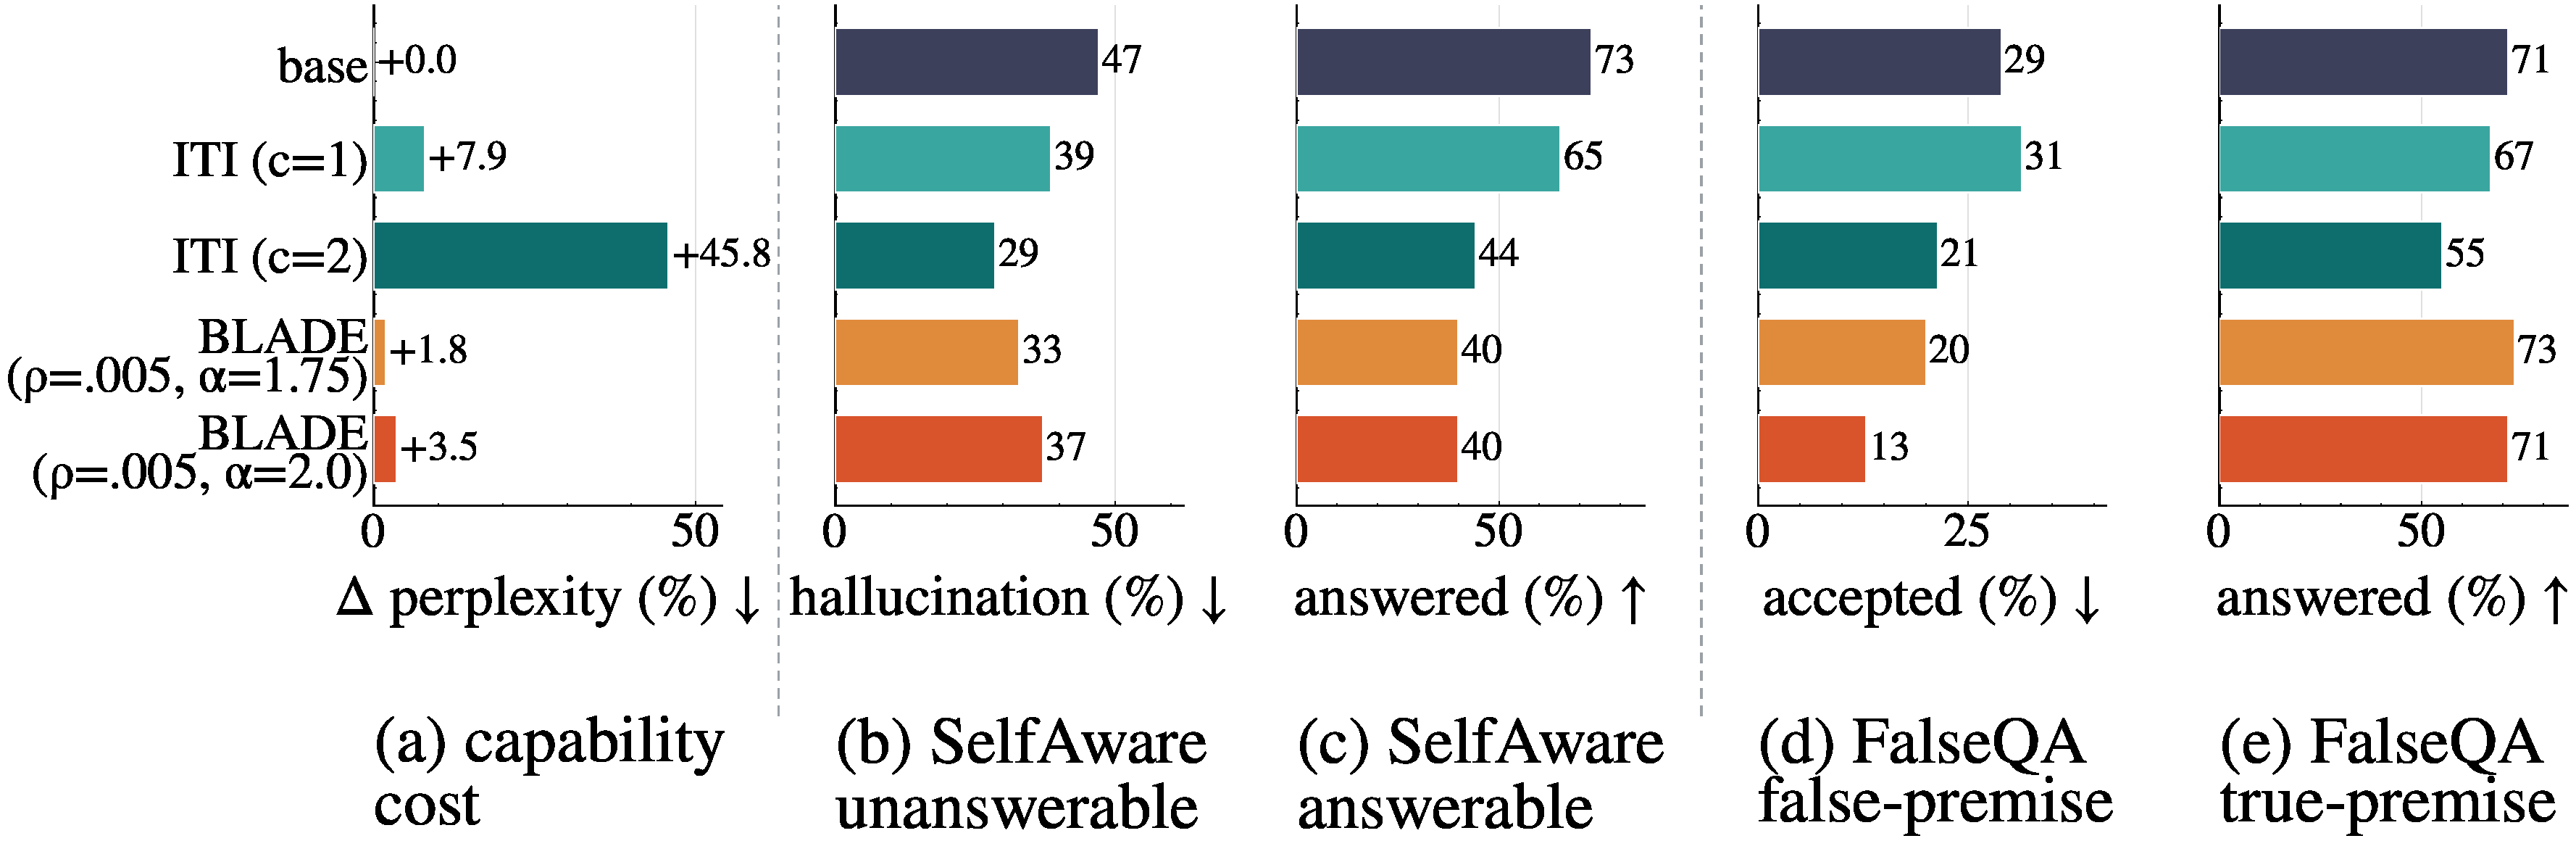
\includegraphics[width=\textwidth]{figures/uncertainty_method_cmp_llama.pdf}
  \caption{\textbf{Llama-3.2-3B-Instruct: BLADE vs.\ ITI}~\citep{li2023iti} (doses re-swept for the
  smaller model: BLADE $\alpha\in\{1.75,2.0\}$ at $\rho{=}.005$, ITI $c\in\{1,2\}$), same five panels as
  Figure~\ref{fig:umc-qwen4b}; lower is better in (a,\,b,\,d), higher in (c,\,e).}
  \label{fig:umc-llama3b}
\end{figure*}

\paragraph{Benchmarks.}
SelfAware~\citep{selfaware} pairs unanswerable questions (the failure: hallucinating an answer) with
answerable ones (the matched behavior: answering); FalseQA~\citep{falseqa} pairs false-premise questions
(the failure: accepting the premise) with valid-premise ones (the matched behavior: answering). A blind
Opus judge labels every response under the ACT taxonomy with the condition hidden; each SelfAware and
FalseQA split has $n{=}70$ prompts, and the ACT taxonomy assigns each response one of
\{answer, abstain, reject-premise, discuss, mixed\}. Capability cost is the teacher-forced C4 $\Delta$-perplexity
relative to the unedited model, so a negative value means the edit slightly \emph{improves} C4 perplexity.

\paragraph{Setup.}
Both methods are fit on the same certain/uncertain prompt contrast at the last prompt token, so the
comparison isolates the \emph{mechanism}, a sparse static weight edit (BLADE-G, thinking-off on the
thinking-capable Qwen3-4B, layers selected automatically by ELS) versus per-head activation steering (ITI),
rather than the source of the
direction. BLADE is controlled by sparsity $\rho$ and amplification $\alpha$; ITI by a dose $c$ in units
of the per-head projection standard deviation. The two knobs are not commensurable, so doses were
re-swept independently on each model. On Qwen3-4B we swept $\rho\in\{.002,.005,.01,.02\}$ and show two
representative $\alpha{=}1.5$ points; on Llama-3.2-3B we fixed $\rho{=}.005$ and re-swept only
$\alpha$, so the Llama BLADE points are not tuned over sparsity.

\paragraph{Qwen3-4B: a Pareto win for BLADE.}
On Qwen3-4B, BLADE at $(\rho{=}.002,\alpha{=}1.5)$ is a Pareto improvement over ITI at $c{=}2$: it is
no worse on any of the four behaviors---better on two (SelfAware hallucination $21\%$ vs.\ $23\%$,
true-premise answering $76\%$ vs.\ $71\%$) and tied on the other two (SelfAware answering $81\%{=}81\%$,
false-premise acceptance $24\%{=}24\%$)---while being cheaper in perplexity ($-0.6\%$ vs.\ $+3.1\%$).
At $n{=}70$ the individual behavioral gaps are a few cases each, so we read this as a consistent
no-worse-and-cheaper result rather than a large margin. Pushing further, BLADE at $(\rho{=}.02,\alpha{=}1.5)$
matches the failure reduction that ITI reaches only at $c{=}4$ (hallucination $17\%$ vs.\ $20\%$,
false-premise acceptance $20\%{=}20\%$) while preserving more of the matched behaviors (SelfAware
answering $71\%$ vs.\ $67\%$, $+4$\,pp; true-premise answering $73\%$ vs.\ $70\%$, $+3$\,pp), and it does
so at $-0.3\%$ perplexity against ITI's $+29.9\%$. The perplexity axis is where the mechanisms diverge
most sharply: both BLADE points have a \emph{negative} $\Delta$-perplexity, whereas ITI's cost climbs
steeply with dose, from $+3.1\%$ at $c{=}2$ to $+29.9\%$ at $c{=}4$---a ${\sim}30\%$ perplexity increase
to reach failure rates BLADE attains at no perplexity cost. In the wider sweep, raising BLADE to
$\alpha\ge2.0$ cuts the failures harder than any ITI dose we tried but begins to over-abstain on the
answerable splits, so we take $\alpha\approx1.5$ as the selected operating point for this model.

\paragraph{Llama-3.2-3B: a harder testbed with one clean axis.}
Figure~\ref{fig:umc-llama3b} is less favorable to either method, and we report it as such. On
SelfAware neither method finds a clean point: BLADE reduces unanswerable hallucination from $47\%$ to
$33\%$ ($\alpha{=}1.75$) and $37\%$ ($\alpha{=}2.0$), but answerable answering collapses from $73\%$
to $40\%$ at both settings; ITI traces the same steep trade-off, with hallucination $39\%$ and $29\%$
against answering $65\%$ and $44\%$ at $c{=}1$ and $c{=}2$. ITI's capability cost also explodes early
on this model: $c{=}1$ already costs $+8.4\%$ perplexity and $c{=}2$ costs $+46.5\%$, by which point
answering has cratered to $44\%$. BLADE stays modest at $+3.5\%$ ($\alpha{=}1.75$) and $+5.7\%$
($\alpha{=}2.0$). The one clean win is FalseQA. BLADE at $\alpha{=}2.0$ cuts false-premise acceptance
from $29\%$ to $13\%$ while fully preserving true-premise answering ($71\%$, identical to base); ITI
reaches only $21\%$ acceptance at $c{=}2$ and drops true-premise answering to $55\%$. We also note an
honest failure of the mild ITI dose: at $c{=}1$ false-premise acceptance actually \emph{rises} above
base ($29\%\to31\%$) while still paying $+8.4\%$ perplexity. We read FalseQA as the clearer axis on this
model: it is where the interventions produce their most consistent separation, whereas at $n{=}70$
(a single case is $1.4$\,pp) the SelfAware differences are smaller relative to sampling granularity.

\paragraph{Cross-model summary.}
At small scale the model matters. Qwen3-4B tolerates a gentle sparse edit, so BLADE delivers a Pareto
improvement over ITI: lower perplexity \emph{and} no worse on any behavior panel. Llama-3.2-3B trades
more steeply on SelfAware, and there FalseQA is the axis on which BLADE's signature still shows: it
reduces the targeted failure at low perplexity cost (negative on Qwen3-4B, $+3.5$--$5.7\%$ on
Llama-3.2-3B) while preserving the matched behavior---fully so for Llama-3.2-3B FalseQA at $\alpha{=}2.0$
(true-premise answering $71\%$, identical to base)---whereas ITI, among the doses we swept, reaches
comparable failure reduction only with a large perplexity increase or a collapse of answering. The common
thread across both models is the mechanism: where a model has headroom, BLADE's sparse static edit reduces
the target failure at little or no perplexity cost, whereas ITI's per-head activation dose buys the same
reduction only by paying a steep, model-dependent perplexity cost, and at low dose it can even backfire,
as on Llama-3.2-3B at $c{=}1$.
